\section{Overview}

Building on the ClimateTV dataset introduced in Chapter~\ref{ch:intro}, this chapter outlines the methodology for analyzing climate change perceptions using social media data. The approach involves two key components: (1) \textbf{Benchmarking zero-shot and task-specific text models}, and (2) \textbf{Fine-tuning text and image models with soft labels} to enhance the capture of nuanced emotions in tweets and their associated images. Additionally, weakly supervised learning approaches are explored to enhance classification performance. This structured approach ensures addressing key challenges associated with analyzing multimodal social media data, such as linguistic variability, noisy inputs, and the subjective nature of climate change discourse. The methodology is structured as follows:

\begin{enumerate}
    \item \textbf{Data Preparation}: The ClimateTV dataset is pre-processed to ensure high-quality text and image inputs. This includes filtering, language detection, tweet selection criteria, and additional preprocessing steps to standardize data for model evaluation.
    
    \item \textbf{Evaluation Metrics}: Metrics are established to systematically assess the performance of zero-shot and task-specific models as well as fine-tuned models using soft labels, ensuring a fair comparison.
    
    \item \textbf{Benchmarking Zero-Shot and Task-Specific Text Models}: A range of pre-trained text models, both zero-shot and task-specific for emotion classification, are evaluated to identify the most effective approach.
    
    \item \textbf{Fine-Tuning with Soft Labels}: The best-performing text model is leveraged to generate soft labels, which are then used to fine-tune additional text and image models, preserving nuanced emotional signals inferred from tweet replies.
    
    \item \textbf{Weakly Supervised Learning}: Weakly supervised techniques are explored to enhance classification performance.
\end{enumerate}


\section{Data Preparation}

\subsection{Data Filtering}
\begin{enumerate}
    \item \textbf{Temporal Filtering}: To capture temporal variations in climate change discourse, this work focuses on the months of \textbf{February and August 2019} from ClimateTV.
    \item \textbf{Language Filtering}:
    \begin{itemize}
        \item \textbf{Primary Tweets}: The \texttt{papluca/xlm-roberta-base-language-detection} model from Hugging Face \cite{papluca_xlm_roberta_base_language_detection} which is a fine-tuned variant of the XLM-RoBERTa \cite{DBLP:journals/corr/abs-1911-02116} classified tweet languages. Only English tweets were retained.
        \item \textbf{Replies}: Replies were pre-translated in the ClimateTV dataset to English.
    \end{itemize}
\end{enumerate}

\subsection{Pre-processing}
\begin{enumerate}
    \item \textbf{Text Cleaning}:
    \begin{itemize}
        \item Removed URLs, hashtags, and user mentions using regex patterns.
        \item Retained emojis and punctuation to preserve sentiment cues.
    \end{itemize}
    \item \textbf{Multimodal Alignment}:
    \begin{itemize}
        \item Paired tweets with their corresponding replies and images using tweet IDs.
        \item Removed orphaned entries (e.g., tweets without replies or images).
    \end{itemize}
\end{enumerate}

\subsection{Final Dataset Statistics}

Table \ref{tab:dataset_stats} presents the final dataset statistics after pre-processing the data between February and August 2019.

\begin{table}[h!]
\centering
\begin{tabular}{lcc}
\toprule
Metric                & February 2019 & August 2019 \\
\midrule
Total Tweets          & 1,774          & 7,769      \\
English Tweets        & 1,673         & 7,345      \\
Replies               & 12,616        & 51,147     \\
Images                & 1,673         & 7,345      \\
\bottomrule
\end{tabular}
\caption{Dataset Statistics for February and August 2019.}
\label{tab:dataset_stats}
\end{table}

\noindent
This pre-processing ensures a focused, high-quality corpus for analyzing climate change perceptions while addressing linguistic and temporal complexities.

\section{Evaluation Metrics}

This research uses two sets of metrics: those that assess ranking performance for pre-trained models (including both zero-shot and task-specific models) and those that measure distributional accuracy when models are fine-tuned with soft labels. 

\subsection{Evaluation Metrics for Zero-Shot and Task-Specific Models}
\label{subsec:pretrained-metrics}

\paragraph{Exact Match (EM) Accuracy:}  
Measures the percentage of predictions for which the top-ranked label matches the ground truth. This provides a strict indicator of precision, especially for unambiguous classes.

\paragraph{Top-3 Accuracy:}  
Calculates the fraction of instances where the correct label appears among the top three predictions. This reflects real-world recommendation scenarios where multiple plausible labels can be acceptable.

\paragraph{Ranked Score (RS):}  
This metric assigns a weighted score to each prediction, giving higher importance to correct labels that appear earlier in the ranked list. Specifically, if a correct label is found at rank \( r \), it receives a score of  \( \frac{1}{\log_2(r+1)} \) . This formulation ensures that models are rewarded for ranking relevant classes higher, thereby emphasizing the importance of correctly prioritizing relevant predictions.

\paragraph{Normalized Discounted Cumulative Gain (NDCG@3):}  
Compares the predicted ranking with the ideal ranking, truncated to the top three positions. This standard information retrieval metric highlights the importance of correctly ordering the most relevant labels.
\begin{equation}
\text{NDCG@3} = \frac{\sum_{i=1}^{3} \frac{\text{rel}_i}{\log_2(i+1)}}{\sum_{i=1}^{3} \frac{\text{rel}_i^{\text{ideal}}}{\log_2(i+1)}}
\end{equation}

where $\text{rel}_i$ represents the relevance score of the item at rank $i$, and $\text{rel}_i^{\text{ideal}}$ denotes the relevance score in the ideal ranking (i.e., sorted in decreasing order of relevance).

\subsection{Fine-Tuning with Soft Labels Evaluation Metrics}

The following metrics evaluate how closely the predicted probability distributions align with the target distributions.


\paragraph{Cosine Similarity:}  
Measures the cosine of the angle between predicted and target probability vectors. This captures directional alignment and is particularly useful for high-dimensional or multi-label tasks. It is computed as:
\begin{equation}
    \text{Cosine Similarity} = \frac{\sum_{i} P(i) Q(i)}{\sqrt{\sum_{i} P(i)^2} \sqrt{\sum_{i} Q(i)^2}}
\end{equation}

\paragraph{Kullback--Leibler Divergence (KLDiv):}  
Quantifies how one probability distribution $Q$ diverges from a true distribution $P$:
\begin{equation}
    D_{\mathrm{KL}}(P \parallel Q) = \sum_{i} P(i) \log \frac{P(i)}{Q(i)}
\end{equation}
It penalizes overconfident misclassifications, which is critical when working with noisy labels.

\paragraph{Mean Squared Error (MSE):}  
Computes the average squared difference between predicted probabilities $Q(i)$ and target probabilities $P(i)$:
\begin{equation}
    \mathrm{MSE} = \frac{1}{N} \sum_{i=1}^{N} \bigl(P(i) - Q(i)\bigr)^2
\end{equation}
MSE is sensitive to large deviations and helps maintain proper probability calibration, reducing the risk of assigning very high probabilities to rare classes.

\paragraph{Ranking-score:}
Finally, to identify the best-performing experiments, we aggregated the mean values of the metrics described above. To standardize the evaluation, we normalized the metrics by preserving Cosine Similarity and inverting MSE and KL Divergence, ensuring higher values indicate better performance. A final ranking score was computed as the sum of these normalized metrics, and experiments were ranked accordingly. This approach provides a robust comparison, enabling the selection of the most effective configurations for further analysis.
\begin{equation}
\text{Ranking-score} = \text{Cosine Similarity} + (1 - \text{MSE}) + (1 - \text{KLDiv})
\end{equation}


\section{Benchmarking Zero-Shot and Task-Specific Text Models}

This section outlines the approach to evaluating and adapting text models for emotion classification in climate-change discourse. Two main categories of models are considered: (1) \textbf{Zero-shot models}, which are general-purpose models applied to this task without prior fine-tuning, and (2) \textbf{Task-specific models} that had been pre-fine-tuned for emotion detection.

\subsection{Dataset and Annotation}

To establish a ground-truth evaluation dataset, \textbf{99 English replies} are sampled from the corpus and manually assigned a single emotion label to each, following Ekman’s six basic emotions—\textit{anger}, \textit{disgust}, \textit{fear}, \textit{joy}, \textit{sadness}, and \textit{surprise}. The label distribution is summarized in Table~\ref{tab:manual_label_distribution}.

\begin{table}[ht]
    \centering
    \begin{tabular}{|c|c|}
        \hline
        \textbf{Manual Label} & \textbf{Count} \\
        \hline
        Anger     & 33 \\
        Joy       & 16 \\
        Disgust   & 15 \\
        Fear      & 13 \\
        Sadness   & 12 \\
        Surprise  & 10 \\
        \hline
    \end{tabular}
    \caption{Distribution of Manual Emotion Labels}
    \label{tab:manual_label_distribution}
\end{table}

\subsection{Models}

The five models benchmarked are chosen for either their zero-shot classification capabilities or their task-specific fine-tuning on Twitter emotion detection:

\begin{enumerate}
    \item \texttt{facebook/bart-large-mnli} \cite{lewis2019bartdenoisingsequencetosequencepretraining}
    \begin{itemize}
        \item A BART model trained for Natural Language Inference (NLI).
        \item Used in a \textbf{zero-shot} classification setting, employing an entailment-based approach \cite{DBLP:journals/corr/abs-1909-00161}.
    \end{itemize}
    
    \item \texttt{MoritzLaurer/mDeBERTa-v3-base-xnli-multilingual-nli-2mil7} \cite{laurer_less_2022}
    \begin{itemize}
        \item A multilingual DeBERTa model trained on cross-lingual NLI tasks.
        \item Enables \textbf{zero-shot} classification across different languages.
    \end{itemize}
    
    \item \texttt{MoritzLaurer/deberta-v3-large-zeroshot-v2.0} \cite{laurer_building_2023}
    \begin{itemize}
        \item A high-performing DeBERTa model fine-tuned specifically for robust \textbf{zero-shot} classification.
    \end{itemize}
    
    \item \texttt{cardiffnlp/twitter-roberta-base-emotion-latest} \cite{antypas2023supertweetevalchallengingunifiedheterogeneous}
    \begin{itemize}
        \item Built on a \textbf{RoBERTa-base} architecture.
        \item Fine-tuned for \textbf{emotion detection on Twitter}, aligning well with our dataset.
        \item Part of the \textbf{SuperTweetEval} benchmark, trained on 154M tweets.
    \end{itemize}
    
    \item \texttt{cardiffnlp/twitter-roberta-large-emotion-latest} \cite{antypas2023supertweetevalchallengingunifiedheterogeneous}
    \begin{itemize}
        \item A \textbf{RoBERTa-large} variant of the above model with greater capacity for contextual reasoning.
        \item Also fine-tuned on Twitter data for emotion detection.
    \end{itemize}
\end{enumerate}

\subsection{Label Mapping to Ekman’s Six Emotions}
\label{subsubsec:ekman}

The CardiffNLP RoBERTa models originally predict emotions across 11 categories (e.g., love, trust, optimism, anticipation). However, to align with the manually annotated dataset, which follows Ekman’s six basic emotions (anger, disgust, fear, joy, sadness, surprise), a mapping is applied to consolidate the predictions into these six categories. This transformation is essential for a direct and meaningful evaluation against the annotated dataset.
\newline

\begin{table}[ht]
    \centering
    \begin{tabular}{|c|l|}
        \hline
        \textbf{Primary Emotion (Ekman)} & \textbf{Mapped Emotions (Original-11)} \\
        \hline
        Anger     & Anger \\
        Disgust   & Disgust \\
        Fear      & Fear \\
        Joy       & Joy, Love, Optimism, Trust \\
        Sadness   & Sadness \\
        Surprise  & Anticipation, Surprise \\
        \hline
    \end{tabular}
    \caption{Mapping of Emotions into Ekman Categories.}
    \label{tab:emotion_mapping}
\end{table}

Table~\ref{tab:emotion_mapping} illustrates the mapping process, where semantically similar emotions are grouped based on shared affective characteristics. For example, love, trust, and optimism are combined under joy due to their common positive valence. Similarly, anticipation, which often carries an element of unpredictability, is merged with surprise.


\subsection{Evaluation Setup}
\label{subsec:eval}

Each model was evaluated in two ways:

\paragraph{1) Primary Evaluation (Standard Metrics)} 
All 99 samples were fed into each model, which returned a single emotion label per sample. The metrics described in Section~\ref{subsec:pretrained-metrics} were computed.

\paragraph{2) Secondary Evaluation (Confidence Filtering)} 
Low-confidence predictions were filtered out by retaining only those with a confidence score above 0.9. This step measured: 
\begin{itemize} 
    \item the proportion of samples that met the threshold, and 
    \item the accuracy of those high-confidence predictions. 
\end{itemize}



\section{Fine-Tuning with Soft Labels} 
\label{sec:finetuning}

This section presents the methodology for fine-tuning unimodal (text-only, image-only) and multimodal (text \& image) models using soft labels. The best performing text model is leveraged to produce label distributions across all replies linked to each parent tweet. For each original tweet, the reply-level probability distributions is aggregated into a single soft label signal by averaging and normalization.
\newline

The resultant aggregated distributions serve as target supervisory signals for fine-tuning, where model parameters are updated by minimizing the Kullback–Leibler (KL) divergence between model outputs and these soft label distributions. This approach enables the model to learn from the aggregated soft label distributions while ensuring that the emotional nuances embedded in the reply-level probability distributions are retained. Figure~\ref{fig:architecture} illustrates the overall framework, including encoder components for each modality and the projection heads that map representations to the soft-label space. Training details regarding objective functions and implementation can be found in Section~\ref{sec:Experimental Setup}.


\subsection{Architectural Overview}
In both cases i.e. Unimodal (Text or Image) and Multimodal, A standard MLP is attached as described below to the encoder for classification, unless specified otherwise. 

\subsubsection*{Projection Head (MLP)}
\begin{itemize}
    \item \textbf{Depth:} 2 layers.
    \item \textbf{Hidden Dimension:} 512.
    \item \textbf{Activation:} ReLU.
    \item \textbf{Output Layer:} Produces $6$ class probabilities (soft labels).
\end{itemize}


\begin{figure}[ht]
    \centering
    \begin{minipage}{0.49\textwidth}
        \centering
        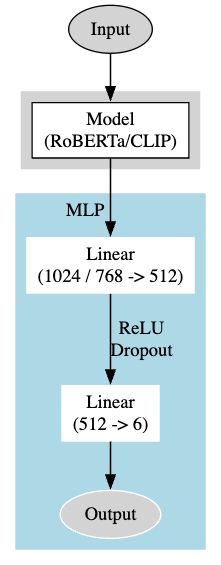
\includegraphics[height=0.5\textheight]{images/unimodal.png}
        \caption{Single Modality Architecture}
        \label{fig:arch1}
    \end{minipage}
    \hfill
    \begin{minipage}{0.49\textwidth}
        \centering
        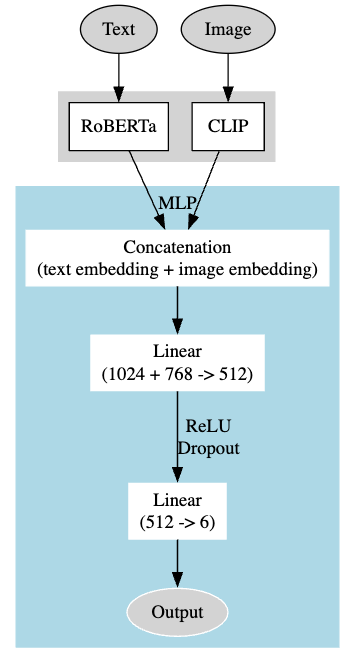
\includegraphics[height=0.5\textheight]{images/multimodal.png}
        \caption{Multimodal Fusion Architecture}
        \label{fig:arch2}
    \end{minipage}
    \caption{Finetuning setup with Base MLP.}
    \label{fig:architecture}
\end{figure}

\subsubsection*{Unimodal-Text (Figure~\ref{fig:arch1})}
Uses a \textbf{Cardiffnlp RoBERTa-Large} encoder to produce text embeddings (1024-dim), followed by the standard projection head.

\subsubsection*{Unimodal-Image (Figure~\ref{fig:arch1})}
Uses a \textbf{CLIP ViT-L/14} encoder to extract image embeddings (768-dim), again followed by the standard projection head.

\subsubsection*{Multimodal Fusion (Figure~\ref{fig:arch2})}
Combines text and image encoders from both unimodal settings in parallel. Text embeddings and image embeddings are concatenated. This fused representation (1792-dim) is passed to the standard projection head. For multimodal experiments, Many fine-tuned variations are tested. The details are:

\begin{itemize}
\item  \textbf{Encoder Tuning}
\begin{itemize}
    \item \textbf{Frozen text encoder:} Only freeze text encoder weights, fine-tune MLP and image encoder.
    \item \textbf{Frozen image encoder:} Only freeze image encoder weights, fine-tune MLP and text encoder.
    \item \textbf{Both encoders frozen:} Freeze both encoder weights, only fine-tune MLP.
    \item \textbf{Full fine-tune:} Fine-tune MLP and both encoders.
    \item \textbf{Staggered-unfreezing:} Unfreeze image encoder weights after 2 epochs and unfreeze text encoder weights after 4 epochs. 
\end{itemize}


\item \textbf{MLP variations}
\begin{itemize}
    \item Standard Projection Head (Figure~\ref{fig:arch2}).
    \item Deeper (3-layer) MLP with ReLU Activation (hidden sizes 1024 and 512).
    \item Deeper (3-layer) MLP with GELU Activation (hidden sizes 1024 and 512).
\end{itemize}



\item \textbf{Fusion strategies}
\begin{itemize}
    \item Late Fusion - Concatenation of final layer embeddings of text and image models (Figure~\ref{fig:arch2}).
    \item Residual Fusion (Concatenation + Residual Addition) (Figure~\ref{fig:residual}), performed along with staggered-unfreezing.
\end{itemize}
\end{itemize}

\begin{figure}[ht]
    \centering
    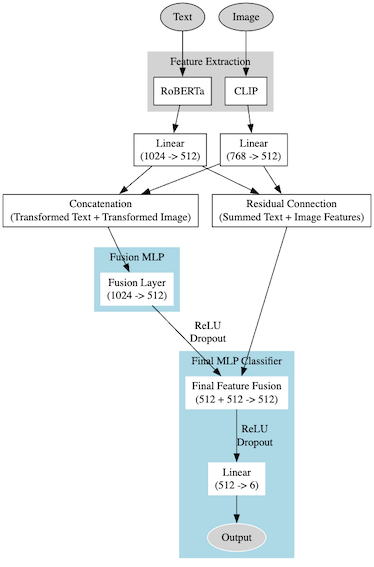
\includegraphics[height=0.6\textheight]{images/residual.png}
    \caption{Multimodal Residual fusion architecture.}
    \label{fig:residual}
\end{figure}



All experiments are conducted on data from two distinct time intervals (February and August) for temporal robustness. These choices are combined systematically resulting in 320 unique experiment configurations (1280 in total for 2 datasets and 2 seeds).
\newline


A summary of the main architectural variations is given in Table~\ref{tab:architectural_variations}.
\newline

\begin{table}[ht]
    \centering
    \resizebox{\textwidth}{!}{%
    \begin{tabular}{lccc}
        \toprule
        \textbf{Component} & \textbf{Text-Based} & \textbf{Image-Based} & \textbf{Multimodal} \\
        \midrule
        Model & RoBERTa-large & CLIP ViT-L/14 & RoBERTa (Large/Base) + CLIP ViT-L/14 \\
        Input & Max 512 tokens & 224 × 224 pixels & Text: 512 tokens, Image: 224 × 224 \\
        Embedding Dim & 1024 & 768 & 1792 \\
        MLP Depth & 2 layers & 2 layers & 2 or 3 layers \\
        Hidden Sizes & 512 & 512 & 1024, 512 (3-layer MLP) \\
        Activation & ReLU & ReLU & ReLU or GELU \\
        Tuning Mode & Frozen or Fine-tuned & Frozen or Fine-tuned & Frozen, Fine-tuned or Staggered, \\
        Fusion Strategy & N/A & N/A & Concatenation / Residual Fusion \\
        \bottomrule
    \end{tabular}%
    }
    \caption{Architectural Variations}
    \label{tab:architectural_variations}
\end{table}

This approach of fine-tuning contrasts with baseline models, which in this study are as follows:

\begin{itemize}
    \item For the \textbf{text-based approach}, the baseline model is the task-specific \textbf{CardiffNLP RoBERTa-Large}.
    \item For the \textbf{image-based approach}, the baseline model is \textbf{CLIP ViT-L/14},  which is used in a zero-shot setting.
    \item For the \textbf{multimodal approach}, the baseline predictions are obtained by averaging the outputs from these two unimodal baseline models.
\end{itemize}


\subsection{Experimental Setup}
\label{sec:Experimental Setup}
This section details the computing environment, hyperparameter selection, reproducibility measures, and monitoring tools used for the experiments.

\subsection*{Hardware and Software Configuration}
\begin{itemize}
    \item \textbf{Hardware:} Two NVIDIA RTX A6000 GPUs with 48~GB VRAM each.
    \item \textbf{Programming Language:} Python 3.9
    \item \textbf{Key Libraries:}
    \begin{itemize}
        \item PyTorch 2.5.0 with CUDA 11.8
        \item HuggingFace Transformers 4.44.2
        \item NumPy 1.26.4, pandas 2.2.2
        \item scikit-learn 1.5.1 for evaluation metrics
        \item TensorBoard 2.18.0 provided real-time loss and accuracy curves
    \end{itemize}
\end{itemize}

\subsection*{Training Configuration and Hyperparameters}

\begin{itemize}
    \item \textbf{Objective Function:} KL divergence to match soft-label distributions.
    \item \textbf{Optimizers:} Compared Adam vs. AdamW (decoupled weight decay $\lambda=0.01$), with $\beta_1=0.9$, $\beta_2=0.999$.
    \item \textbf{Learning Rates:} \{ $1 \times 10^{-5}$, $5 \times 10^{-6}$ \}.
    \item \textbf{Batch Size:} Typically 16 per GPU.
    \item \textbf{Epochs:} 2, 5 and 10
    \item \textbf{Regularization:}
    \begin{itemize}
        \item Dropout \{0.3, 0.5\} within MLP layers.
        \item Weight decay (AdamW).
    \end{itemize}
    \item \textbf{Data Split:} A 70-20-10 split was used for training, validation, and testing, respectively.
\end{itemize}

\subsection*{Reproducibility Protocol}
\begin{itemize}
    \item All experiments are conducted using two distinct random seeds (42 and 7) to ensure reproducibility.
    \item Randomness is controlled by setting the same seed for Python's random module, NumPy, PyTorch, and CUDA operations.
    \item Identical initialization and data splits are maintained across all runs.
\end{itemize}


\section{Weakly Supervised Learning}

In this section, two weakly supervised approaches were explored to improve model performance. The first approach builds upon \cite{gera_zero-shot_2022}, which proposed a self-training framework to enhance zero-shot classification by iteratively fine-tuning models on their own high-confidence predictions. The second approach focuses on loss re-weighting, where we integrate confidence scores into the loss function to prioritize reliable pseudo-labels while mitigating the impact of noise.

\subsection{Zero-Shot Classification Boost with Self-training}
As outlined in Section \ref{sec:weakly_supervised_back}, \cite{gera_zero-shot_2022} proposed a self-training framework. Their approach addresses the scarcity of labelled data by leveraging unlabeled corpora and class names alone, aligning with our goal of "classifying tweets into distinct emotion categories without task-specific labels". 

\subsubsection*{Reproduction of Gera et al.’s Methodology}
To validate the reproducibility of the original study, we reimplemented their workflow as follows:

\subsubsection*{Model and Dataset Selection}
\begin{itemize}
    \item The same off-the-shelf NLI models (RoBERTa-large, DeBERTa-v3) and datasets \textit{(AG’s news \cite{DBLP:journals/corr/ZhangZL15} and ISEAR \cite{Shao2015UniversalityVC})} were used as described in the original work.
    \item Weak supervision signals were derived solely from class names and unlabelled text, mirroring the zero-shot setup.
\end{itemize}

\subsubsection*{Self-Training Protocol}
\begin{itemize}
    \item \textbf{Pseudo-Label Generation:} For each dataset, pseudo-labels by selecting the model’s most confident predictions were generated (threshold: $\tau = 0.9$, as in the original study).
    \item \textbf{Token Masking:} The token masking heuristic to mask tokens with high semantic similarity to class names (using cosine similarity over SBERT embeddings) was implemented.
    \item \textbf{Fine-Tuning:} Models were iteratively fine-tuned on pseudo-labeled batches (batch size: 8) for $K = 2$ iterations, retaining the original learning rate ($2 \times 10^{-5}$) and optimizer (AdamW).
\end{itemize}

\noindent
The framework was adapted to our task of \textit{classifying tweets into distinct emotion categories}.

\subsubsection*{Adaptations to the Self-Training Pipeline}
\begin{itemize}
    \item \textbf{Class Name Prompt Engineering:} To improve pseudo-label quality, we reformulated class names into natural language hypotheses (e.g., "The emotion in this text is joy" instead of "joy").
    \item \textbf{Cross-Task Sampling:} Since our task lacks related labelled datasets, we limited self-training to in-domain pseudo-labels, avoiding the cross-task degradation noted in \cite{gera_zero-shot_2022}.
\end{itemize}


\subsection{Loss Re-weighting}  
\label{sec:loss_reweighting}  

To mitigate label noise from weak supervision, a confidence-based loss re-weighting strategy was implemented as described in sub-section \ref{subsubsec:loss_adjust}. This approach adjusts the influence of each training example based on confidence scores derived from the initial label generation process.  

\subsubsection{Implementation}  

This method consists of three key components:  

\begin{itemize}
    \item \textbf{Confidence-Weighted Loss Function}: The standard cross-entropy loss was modified to incorporate confidence scores as multiplicative weights. This ensured that higher-confidence samples contributed more to the learning process, while lower-confidence samples had a reduced impact. Model output probabilities were used as confidence scores.

    \item \textbf{Data Integration Pipeline}: The training dataset combined weak labels, raw text, and confidence scores, represented as:  

    \begin{equation}
        \mathcal{D} = \{(\mathbf{x}_i, \tilde{y}_i, c_i)\}_{i=1}^N
    \end{equation}

    where $\tilde{y}_i$ denotes weak labels, and $c_i \in [0,1]$ represents the assigned confidence score.  

    \item \textbf{Adaptive Training Protocol}: BERT-base model was fine-tuned using a structured approach:  
    \begin{itemize}
        \item Applied class-balanced sampling when enabled  
        \item Used the AdamW optimizer with a learning rate of $2\times10^{-5}$  
        \item Implemented early stopping based on validation performance  
    \end{itemize}
\end{itemize}  

\subsubsection{Theoretical Basis}  

This method aligns with a noise-robust learning objective:  

\begin{equation}
    \min_\theta \sum_{i=1}^N c_i \cdot \ell(f_\theta(\mathbf{x}_i), \tilde{y}_i)
\end{equation}

where $\ell$ is the cross-entropy loss, and $c_i$ acts as a weighting factor. This formulation prioritizes high-confidence samples while minimizing the influence of potentially incorrect labels.  








